\documentclass[a4paper,12pt]{article}
%%% Работа с русским языком % для pdfLatex
\usepackage{cmap}					% поиск в~PDF
\usepackage{mathtext} 				% русские буквы в~фомулах
\usepackage[T2A]{fontenc}			% кодировка
\usepackage[utf8]{inputenc}			% кодировка исходного текста
\usepackage[english,russian]{babel}	% локализация и переносы
\usepackage{indentfirst} 			% отступ 1 абзаца

%%% Работа с русским языком % для XeLatex
%\usepackage[english,russian]{babel}   %% загружает пакет многоязыковой вёрстки
%\usepackage{fontspec}      %% подготавливает загрузку шрифтов Open Type, True Type и др.
%\defaultfontfeatures{Ligatures={TeX},Renderer=Basic}  %% свойства шрифтов по умолчанию
%\setmainfont[Ligatures={TeX,Historic}]{Times New Roman} %% задаёт основной шрифт документа
%\setsansfont{Comic Sans MS}                    %% задаёт шрифт без засечек
%\setmonofont{Courier New}
%\usepackage{indentfirst}
%\frenchspacing

%%% Дополнительная работа с математикой
\usepackage{amsfonts,amssymb,amsthm,mathtools}
\usepackage{amsmath}
\usepackage{icomma} % "Умная" запятая: $0,2$ --- число, $0, 2$ --- перечисление
\usepackage{upgreek}

%% Номера формул
%\mathtoolsset{showonlyrefs=true} % Показывать номера только у тех формул, на которые есть \eqref{} в~тексте.

%%% Страница
\usepackage{extsizes} % Возможность сделать 14-й шрифт

%% Шрифты
\usepackage{euscript}	 % Шрифт Евклид
\usepackage{mathrsfs} % Красивый матшрифт

%% Свои команды
\DeclareMathOperator{\sgn}{\mathop{sgn}} % создание новой конанды \sgn (типо как \sin)
\usepackage{csquotes} % ещё одна штука для цитат
\newcommand{\pd}[2]{\ensuremath{\cfrac{\partial #1}{\partial #2}}} % частная производная
\newcommand{\abs}[1]{\ensuremath{\left|#1\right|}} % модуль
\renewcommand{\phi}{\ensuremath{\varphi}} % греческая фи
\newcommand{\pogk}[1]{\!\left(\cfrac{\sigma_{#1}}{#1}\right)^{\!\!\!2}\!} % для погрешностей

% Ссылки
\usepackage{color} % подключить пакет color
% выбрать цвета
\definecolor{BlueGreen}{RGB}{49,152,255}
\definecolor{Violet}{RGB}{120,80,120}
% назначить цвета при подключении hyperref
\usepackage[unicode, colorlinks, urlcolor=blue, linkcolor=blue, pagecolor=blue, citecolor=blue]{hyperref} %синие ссылки
%\usepackage[unicode, colorlinks, urlcolor=black, linkcolor=black, pagecolor=black, citecolor=black]{hyperref} % для печати (отключить верхний!)


%% Перенос знаков в~формулах (по Львовскому)
\newcommand*{\hm}[1]{#1\nobreak\discretionary{}
	{\hbox{$\mathsurround=0pt #1$}}{}}

%%% Работа с картинками
\usepackage{graphicx}  % Для вставки рисунков
\graphicspath{{images/}{images2/}}  % папки с картинками
\setlength\fboxsep{3pt} % Отступ рамки \fbox{} от рисунка
\setlength\fboxrule{1pt} % Толщина линий рамки \fbox{}
\usepackage{wrapfig} % Обтекание рисунков и таблиц текстом
\usepackage{multicol}

%%% Работа с таблицами
\usepackage{array,tabularx,tabulary,booktabs} % Дополнительная работа с таблицами
\usepackage{longtable}  % Длинные таблицы
\usepackage{multirow} % Слияние строк в~таблице
\usepackage{caption}
\captionsetup{labelsep=period, labelfont=bf}

%%% Оформление
\usepackage{indentfirst} % Красная строка
%\setlength{\parskip}{0.3cm} % отступы между абзацами
%%% Название разделов
\usepackage{titlesec}
\titlelabel{\thetitle.\quad}
\renewcommand{\figurename}{\textbf{Рис.}}		%Чтобы вместо figure под рисунками писал "рис"
\renewcommand{\tablename}{\textbf{Таблица}}		%Чтобы вместо table над таблицами писал Таблица

%%% Теоремы
\theoremstyle{plain} % Это стиль по умолчанию, его можно не переопределять.
\newtheorem{theorem}{Теорема}[section]
\newtheorem{proposition}[theorem]{Утверждение}

\theoremstyle{definition} % "Определение"
\newtheorem{definition}{Определение}[section]
\newtheorem{corollary}{Следствие}[theorem]
\newtheorem{problem}{Задача}[section]

\theoremstyle{remark} % "Примечание"
\newtheorem*{nonum}{Решение}
\newtheorem{zamech}{Замечание}[theorem]

%%% Правильные мат. символы для русского языка
\renewcommand{\epsilon}{\ensuremath{\varepsilon}}
\renewcommand{\phi}{\ensuremath{\varphi}}
\renewcommand{\kappa}{\ensuremath{\varkappa}}
\renewcommand{\le}{\ensuremath{\leqslant}}
\renewcommand{\leq}{\ensuremath{\leqslant}}
\renewcommand{\ge}{\ensuremath{\geqslant}}
\renewcommand{\geq}{\ensuremath{\geqslant}}
\renewcommand{\emptyset}{\varnothing}

\usepackage{bm} %жирный греческий шрифт
%\usepackage{ulem}
\usepackage{enumitem}
\usepackage{float}

\graphicspath{{images}}

\title{Laba}
\author{Георгий Демьянов}
\date{today}
\usepackage[left=1.27cm,right=1.27cm,top=2cm,bottom=2cm]{geometry}
\usepackage{bigstrut}
\usepackage{comment}
\usepackage{makecell}
\usepackage{microtype}
\usepackage{gensymb}
\newcommand{\figref}[1]{(рис. \ref{#1})}
\usepackage{float} % Ставит рисунки и таблицы в СТРОГО нужное место с помощью команды {H}

\begin{document}
\begin{titlepage}
\begin{center} 
 
\large Московский физико-технический институт\\
Факультет молекулярной и химической физики\\
\vspace{7cm}
\Large Лабораторная работа \\по курсу \\ Физические методы исследований\\
\textbf{\Huge <<ИЗМЕРЕНИЕ ВРАЩАТЕЛЬНОЙ И КОЛЕБАТЕЛЬНОЙ ТЕМПЕРАТУР\\ В
	ГАЗОВОМ РАЗРЯДЕ\\
	ПО СПЕКТРУ МОЛЕКУЛЫ >>}\\
\end{center} 

\vspace{5cm}
{\par \raggedleft \large \emph{Выполнили:}\\ студенты 3 курса\\ 642 группы ФМХФ\\ Демьянов Георгий Сергеевич \\ Шадымов Владимир Александрович\par}
\begin{center}
\vfill Москва 2019
\end{center}
\end{titlepage}
\newpage
\setcounter{page}{2}
\tableofcontents
\clearpage
%\renewcommand{\baselinestretch}{1.3}
%\begin{center}
	\vspace{0.5cm}
	{\parbox{16cm}
		{\small{\centering{\textbf{Аннотация}\\
					\hspace{0.6cm} 
					В этом отчёте изложены результаты выполнения лабораторной работы «ЯМР-релаксация». Были проделаны измерения времени продольной и поперечной релаксации протонной намагниченности для воды и растворов $MnSO_4$ и $Na_2 SO_4$ различной концентрации. Полученные времена релаксации. Работа выполнялась с использованием ЯМР-релаксометра \textit{Bruker Minispec}.
				}
			}
		}
	}
\end{center}

\textbf{\emph{Цель работы:}}
изучить механизм релаксации ядерной намагниченности и освоить методы измерения продольной и поперечной релаксации протонов.
\section{Теоретическое введение}
\subsection{Суть ЯМР}
Явление ЯМР заключается в резонансном поглощении электромагнитной энергии макроскопической системой ядерных магнитных моментов, помещенных в постоянное внешнее магнитное поле. Ядерные магнитные моменты связаны с наличием у протонов и нейтронов \textit{спинов}.

Энергия $E$ магнитного момента, находящегося в постоянном магнитном поле $\vec{B_0}$, равна
\begin{equation}
\label{E_in_field}
E = - (\vec{\mu}, \vec{B_0}) = -\mu B_0 \cos \theta = - g \beta_N B_0 m_z
\end{equation}
где $\theta$ -- угол между направлениями векторов $\mu$ и $B_0$, а $ m_z $ -- проекция спина на ось $z$, совпадающую с направлением $ B_0 $, $\beta_N = 5.0508 \cdot 10^{-27} \text{Дж}/\text{Тл}$ -- ядерный магнетон, $g$ -- так называемый фактор Ланде, представляющий из себя безразмерную величину (индивидуален для каждого вещества).
Протон имеет спин $ I = 1/2 $, поэтому возможные значения проекции спина на ось квантования равны $ m_z = \pm 1/2 $.

Из (\ref{E_in_field}) следует, что в магнитном поле $B_0$ происходит расщепление на два состояния, имеющие разную энергию.
Между этими уровнями возможны переходы при поглощении кванта электромагнитной энергии определенной частоты -- это и есть суть ЯМР.

\subsection{Уравнение Блоха и радиочастотные импульсы}
В равновесном состоянии суммарная намагниченность $M$ ансамбля спинов, помещенных во внешнее постоянное магнитное поле, ориентируется параллельно направлению приложенного поля. Удобной моделью для описания поведения вектора суммарной намагниченности в магнитном поле является феноменологическая теория Блоха.
\begin{equation}
\label{Bloh_simple}
\dfrac{d \vec{M}(t)}{dt} = \gamma \vec{M}(t) \times \vec{B}(t)
\end{equation}
где $\gamma = \dfrac{2 \pi g \beta_N}{h}$.

При воздействии радиочастотного поля $ \vec{B}_1(t) = \vec{B}_{1m} \sin(\omega t) $, направленного перпендикулярно направлению постоянного магнитного поля $ B_0 $, на систему спинов намагниченность последней будет находиться под воздействием поля $\vec{B}(t) = \vec{B}_1 (t) + \vec{B}_0$.
Действие переменного поля удобно анализировать на основе уравнения Блоха, используя систему координат, вращающуюся с Ларморовой частотой $ \omega_0 = \gamma B_0 $ вокруг направления $z$ постоянного поля. В этой системе уравнение (\ref{Bloh_simple}) без учета релаксации имеет вид:
\begin{equation}
\label{Bloh_rotation}
\dfrac{d \vec{M}(t)}{dt} = \gamma \vec{M}(t) \times \left(\vec{B}(t) - \dfrac{\omega_0}{\gamma} \right)
\end{equation}
Под действием переменного электромагнитного поля с резонансной частотой $ \omega_0 = \gamma B $ вектор намагниченности во вращающейся СК совершает прецессию вокруг вектора $B_1$ поля с угловой частотой $ \omega_1 = \gamma B_1 $. Если переменное магнитное поле действует в течение короткого времени $ \tau_\theta $, то вектор намагниченности повернется на угол:
\begin{equation}
\label{Theta_def}
\theta = \gamma B_1 \tau_\theta
\end{equation}
где $ \theta $ -- угол поворота в радианах, $ \gamma  $ -- гиромагнитное отношение (для ядер $^1$H $ \gamma = 26.75~\cdot~10^7 \text{рад }\text{с}^{-1}\text{Тл}^{-1} $)

Для поворота суммарной намагниченности на заданный угол $\theta$ настраивают амплитуду $ B_1 $ и длительность $ \tau_\theta $ в соответствии с (\ref{Theta_def}). При этом для угла $90 ^{\circ}$ импульс называется \textit{$\pi /2$-импульсом}, а для угла $180 ^{\circ}$ называется \textit{$ \pi $-импульсом}.

\begin{figure}[h]
	\centering
	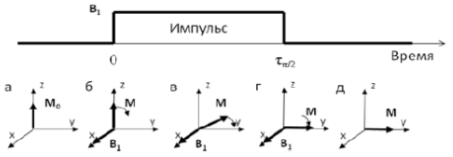
\includegraphics[width=0.7\linewidth]{M-rotation}
	\caption{Поведение суммарной намагниченности под действием $\pi /2$-импульса (вращающаяся СК). \textbf{а} -- до включения; \textbf{б} -- начало действия импульса; \textbf{в} -- поворот намагниченности; \textbf{г} --  окончание действия импульса; \textbf{д} -- прецессия намагниченности вокруг оси $z$ после выключения импульса}
	\label{fig:m-rotation}
\end{figure}


\subsection{Релаксация ядерной намагниченности}
Процесс восстановления суммарной намагниченности к исходному равновесному состоянию называют \textit{релаксацией намагниченности}. Уравнение Блоха с учетом процессов релаксации выглядит следующим образом
\begin{align}
\label{Bloh-relaxaion}
\dfrac{d M_x}{dt} &= \gamma \left[ M_y B_z - M_z B_y\right] - \dfrac{M_x}{T_2} \\
\dfrac{d M_y}{dt} &= \gamma \left[ M_z B_x - M_x B_z\right] - \dfrac{M_y}{T_2} \\
\dfrac{d M_z}{dt} &= \gamma \left[ M_x B_y - M_y B_x\right] - \dfrac{M_z - M_0}{T_1} \\
\end{align}

Решение уравнения Блоха после окончания действия $\pi /2$-импульса выглядит следующим образом:
\begin{align}
\label{Bloh-solution-pi/2}
	\vec{M}(t) = M_0
	\begin{pmatrix}
		0 \\
		e^{-t/T_2} \\
		1 - e^{-t/T_1}
	\end{pmatrix}
\end{align}

\subsection{Механизмы ЯМР-релаксации}
При тепловом движении частиц, имеющих магнитные моменты, возникают локальные магнитные поля, изменяющиеся во времени случайным образом. В спектре их случайных функций поля есть компоненты с частотой ЯМР. Их действие аналогично действию внешнего радиочастотного поля, т.е. переменное локальное поле может вызывать переходы между уровнями энергии спиновой системы. Изменяющееся случайным образом поле $ \vec{B}'(t) $ можно описать с помощью корреляционной функции $ K(\tau) $:
\begin{equation}
\label{korrel_function_def}
K_i (\tau) = \overline{B_i'(t) B_i'(t+\tau)}
\end{equation}
где $ B_i' $ -- одна из компонент флуктуирующего поля, а черта означает усреднение по всевозможным реализациям этого произведения по различным начальным моментам времени $ t $. Значения случайной функции на больших интервалах времени не коррелированы, следовательно, $K(\infty) \rightarrow 0$.

Во многих практически важных случаях $K$ имеет вид:
\begin{equation}
\label{K_exponential}
K(\tau) = \overline{\abs{B'(t)}^2} e^{-\abs{\tau}/\tau_C}
\end{equation}

Спектральная плотность определяется как Фурье-преобразование функции корреляции:
\begin{equation}
\label{Spectre-power-def}
J(\omega) = \int_{-\infty}^{+\infty} K(\tau) e^{-i \omega t} d\tau
\end{equation}

Для нашей экспоненциальной функции:
\begin{equation}
\label{Spectre-power-exp}
J(\omega) = \dfrac{2\tau_C}{1 + \omega^2 \tau_C^2} \overline{\abs{B'(t)}^2}
\end{equation}

Поперечные компоненты локального флуктурирующего поля, направленные вдоль осей $x$ и $ y $ и осциллирующие с резонансной частотой $ \omega_0 $, приводят к спин-решеточной релаксации. Скорость продольной релаксации определяется $J$ на частоте резонанса:
\begin{equation}
\label{T_1-of-J}
\dfrac{1}{T_1} = \gamma^2 J(\omega_0) = \gamma^2 \overline{\abs{B'(t)}^2} \dfrac{2 \tau_C}{1 + \omega_0^2 \tau_C^2}
\end{equation}

Поперечная релаксация определяется:
\begin{enumerate}[label=\alph*)]
	\item компонентами локального поля, изменяющимися с частотами близкими к резонансной -- аналогично спин-решеточной релаксации (спиновая подсистема отдает часть энергии термостату, потом берет обратно);
	\item потерей когерентности прецессии (,,сбой фазы прецессии'') магнитных моментов, образующих вектор намагниченности $ \vec{M} $ из-за изменения частоты ЯМР в переменном поле $ \vec{B}(t) $.
\end{enumerate}

Выражение для скорости поперечной релаксации для системы невзаимодействующих друг с другом спинов в модели невзаимодействующих протонов в изотропном флуктуирующем локальном поле имеет вид:
\begin{equation}
\label{T_2-of-J}
\dfrac{1}{T_2} = \dfrac{1}{2 T_1} + \dfrac{1}{T_2'} = \gamma \overline{\abs{B'(t)}^2} \left(\frac{1}{2} J(\omega_0) + \frac{1}{2} J(0) \right) = \gamma^2 \overline{\abs{B'(t)}^2} \left(\dfrac{\tau_C}{1 + \omega_0^2 \tau_C^2} + \tau_C \right)
\end{equation}

\subsection{Импульсные последовательности}
Практически все современные методики использования ЯМР заключаются в изучении поведения намагниченности системы спинов после воздействия на нее определенной последовательности радиочастотных импульсов.
Простейшим примером является последовательность, состоящая из одного $\pi /2$-импульса. 
После окончания действия радиочастотного импульса, в соответствии с (\ref{Bloh-solution-pi/2}), зависимость поперечной намагниченности от времени во вращающейся системе координат будет определяться соотношением $M_y = M_0 e^{-t/T_2}$.
В лабораторной системе координат временная зависимость поперечной намагниченности будет иметь вид $ M_y' = M_0 e^{-t/T_2} \sin(\omega_0 t) $. 
Данную зависимость, регистрируемую после воздействия $\pi /2$-импульса, называют \textit{сигналом спада свободной индукции} (ССИ).
Фурье-преобразование зависимости $ M_y' (t) $ позволяет получить частотный спектр ЯМР (рис. \ref{fig:fourier-example}).
\begin{figure}[h]
	\centering
	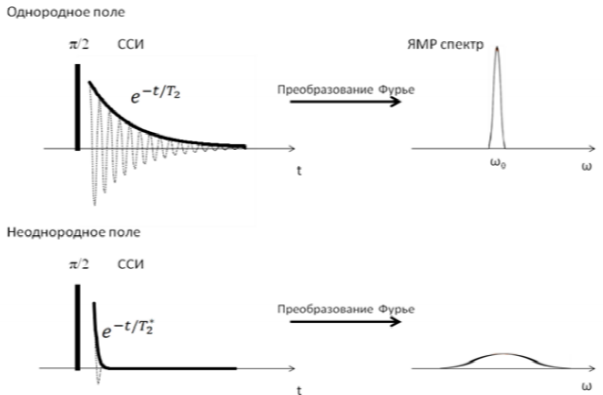
\includegraphics[width=0.7\linewidth]{Fourier-example}
	\caption{Спад свободной индукции после воздействия $\pi /2$-импульса в однородном и неоднородном магнитных полях}
	\label{fig:fourier-example}
\end{figure}

В условиях реального эксперимента постоянное магнитное поле не является идеально однородным в объеме образца. 
Неоднородность поля приводит к тому, что прецессия векторов намагниченности происходит с разными частотами в разных областях пространства. 
Поэтому со временем фазовая когерентность прецессии векторов намагниченности разных частей образца теряется, в результате поперечная компонента суммарной намагниченности образца уменьшается. 
Общая скорость уменьшения поперечной намагниченности ($ 1/T_2^* $), фигурирующая в уравнении Блоха, в неоднородном магнитном поле определяется скоростью поперечной релаксации и потерей фазовой когерентности из-за неоднородности постоянного магнитного поля:
\begin{equation}
\label{T2*_def}
\dfrac{1}{T_2^*} = \dfrac{1}{T_2} + \dfrac{\gamma \Delta B}{2}
\end{equation}
где $ \Delta B $ характеризует неоднородность МП.
Итак, если магнитное поле неоднородно, то регистрировать спектры ЯМР становится невозможно из-за значительного уширения сигналов. Анализ спада свободной индукции после воздействия $ \pi /2 $-импульса в таком поле не даст определить значение $ T_2 $. Для обхода этой проблемы используются специальные импульсные последовательности, основанные на явлении спинового эха Хартмана-Ханна.
% TODO: написать про импульсные последовательности

\subsection{Импульсная последовательность КПМГ для регистрации времени $ T_2 $}
Для регистрации времен поперечной релаксации используется последовательность КПМГ (рис. \ref{fig:2019-02-11}).
\begin{figure}
	\centering
%	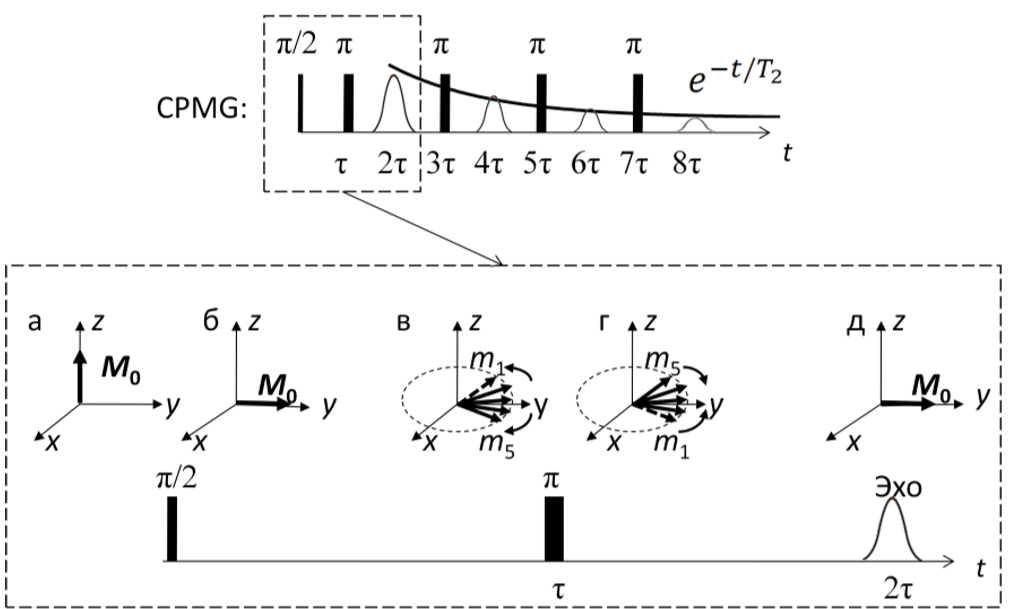
\includegraphics[width=0.7\linewidth]{2019-02-11}
	\caption{}
	\label{fig:2019-02-11}
\end{figure}
Импульсная последовательность КПМГ состоит из одного $\pi /2$ импульса, поворачивающего намагниченность на угол $\pi /2$ вокруг оси x, и серии $\pi$-импульсов, поворачивающих намагниченность на угол $\pi$ вокруг оси y, прикладываемых через определенные промежутки времени (рис. \ref{fig:2019-02-11}). Данная импульсная последовательность основана на наблюдении серии сигналов спинового эха Хартмана–Ханна. В отсутствие процессов поперечной релаксации амплитуда сигналов эха оставалась бы неизменной, а при протекании поперечной релаксации их амплитуда постепенно уменьшается. Время поперечной релаксации $T_2$ определяют из зависимости значения амплитуды сигнала эха M от времени между импульсами $\tau$ и номера сигнала эха n:  
\begin{equation}
\label{eq:T2-def}
M(2n\tau)=M_0 e^{-\dfrac{2n\tau}{T_2}}
\end{equation}

Время $\tau$ обычно выбирается так, чтобы $\tau << T_1$, восстановлением продольной компоненты намагниченности при этом можно пренебречь. 

\subsection{Импульсная последовательность насыщение–восстановление для регистрации времен $T_1$ }
Для регистрации времен продольной релаксации используется импульсная последовательность насыщение–восстановление (рис. \ref{fig:2019-02-111}).
\begin{figure}
	\centering
%	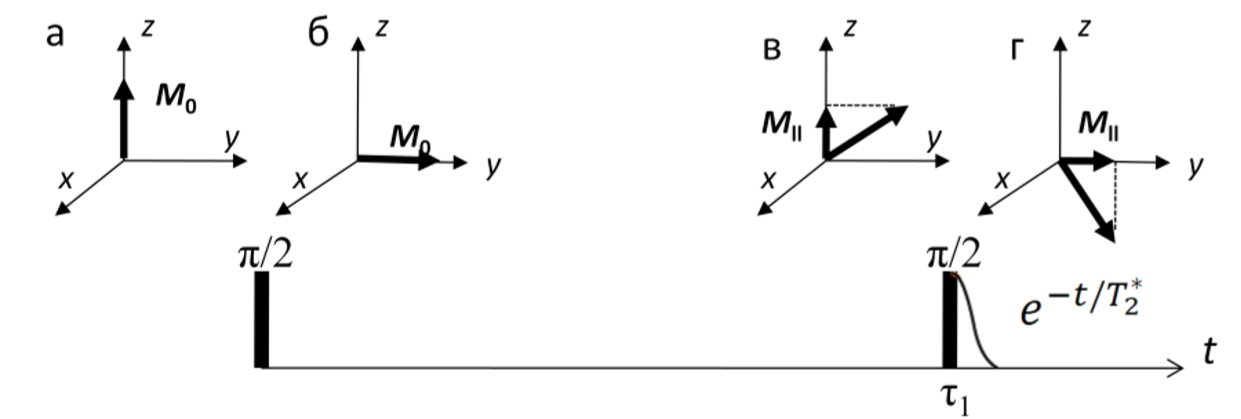
\includegraphics[width=0.7\linewidth]{2019-02-111}
	\caption{}
	\label{fig:2019-02-111}
\end{figure}
Эта последовательность состоит из двух радиочастотных $\pi$/2-импульсов. 
До воздействия первого $\pi$/2 импульса, суммарная намагниченность $M_0$ системы ядер ориентирована параллельно оси $z$, направление которой совпадает с направлением постоянного магнитного поля $B_0$ (рис. \textbf{а}). 
Воздействуя в момент времени $\tau_1$ вторым $\pi$/2-импульсом, можно перевести продольную компоненту намагниченности $M_{||}$ в плоскость $(x, y)$, в которой она может быть измерена (рис. \textbf{г}).
После восстановления равновесия (в течение времени около $5T_1$) данную последовательность повторяют с увеличенным значением интервала между импульсами $\tau_1$. 
Время продольной релаксации $T_1$ определяют по зависимости значения $M_{||}$ от времени между импульсами $\tau_1$ в серии экспериментов с различными значениями $\tau_1$: 
\begin{equation}
\label{eq:T1-def}
M_{||}(\tau_1)= M_0 \left(1-e^{-\dfrac{\tau_1}{T_1}} \right)
\end{equation}
%\newpage
\section{Проведение эксперимента}
В данной работе источником излучения служит тлеющий разряд в воздухе.
Принципиальная схема регистрации излучения представлена на \figref{ust}. Излучение
регистрируется через боковую стенку разрядного отсека плазмотрона. Изображение плазмы в
масштабе 1:4 с помощью линзы из LiF фокусируется на входную щель монохроматора МДР-23.
\begin{figure}[H]
	\begin{center}
		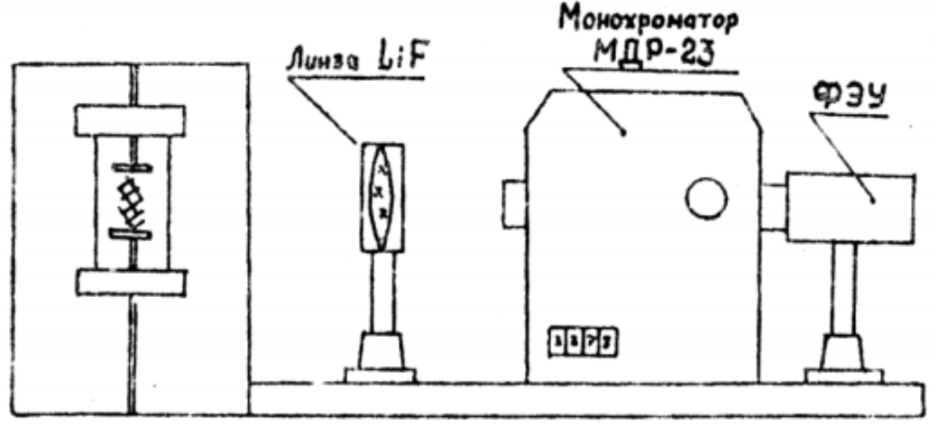
\includegraphics[width=0.65\textwidth]{ystanovka.png}
		\caption{Схема регистрации излучения}
		\label{ust}
	\end{center}	
\end{figure}

В качестве диспергирующего элемента монохроматора используется дифракционная
решетка, имеющая 1200 штрихов на миллиметр (1200 /1). За выходной щелью
монохроматора помешается фотоумножитель ФЭУ-100. Монохроматор МДР-23
используется в составе управляющего измерительного комплекса КСВУ-23, включающего
также ЭВМ ДВК-3, интерфейсные блоки связи ЭВМ с экспериментальной установкой,
усилитель с высокоомным входом, управляемый от ЭВМ источник высокого напряжения
для питания ФЭУ. Конструкция монохроматора позволяет осуществлять сканирование
спектра в автоматическом режиме с заданной скоростью. Дифракционная решетка при
этом поворачивается с помощью шагового двигателя.


Использование воздушной смеси азота и кислорода принципиально, так как при содержании кислорода менее 2 \% в спектре появляются полосы отрицательной ($1^{-}$)-системы ${N_2}^+$, чья интенивность может превосходить интенсивность (2+) системы.  
%\newpage
\section{Обработка результатов измерений}
\subsection{Результаты измерений}
Приведем графики полученных спектров (рис. \ref{full_45}--\ref{full_65}). В день опытов атмосферное давление было равно $p_0 = 750$ торр. По полученным данным проведем идентификацию наблюдаемых полос (табл. \ref{tab:polosi}).
\begin{figure}[H]
	\begin{minipage}{0.45\linewidth}
		\centering
		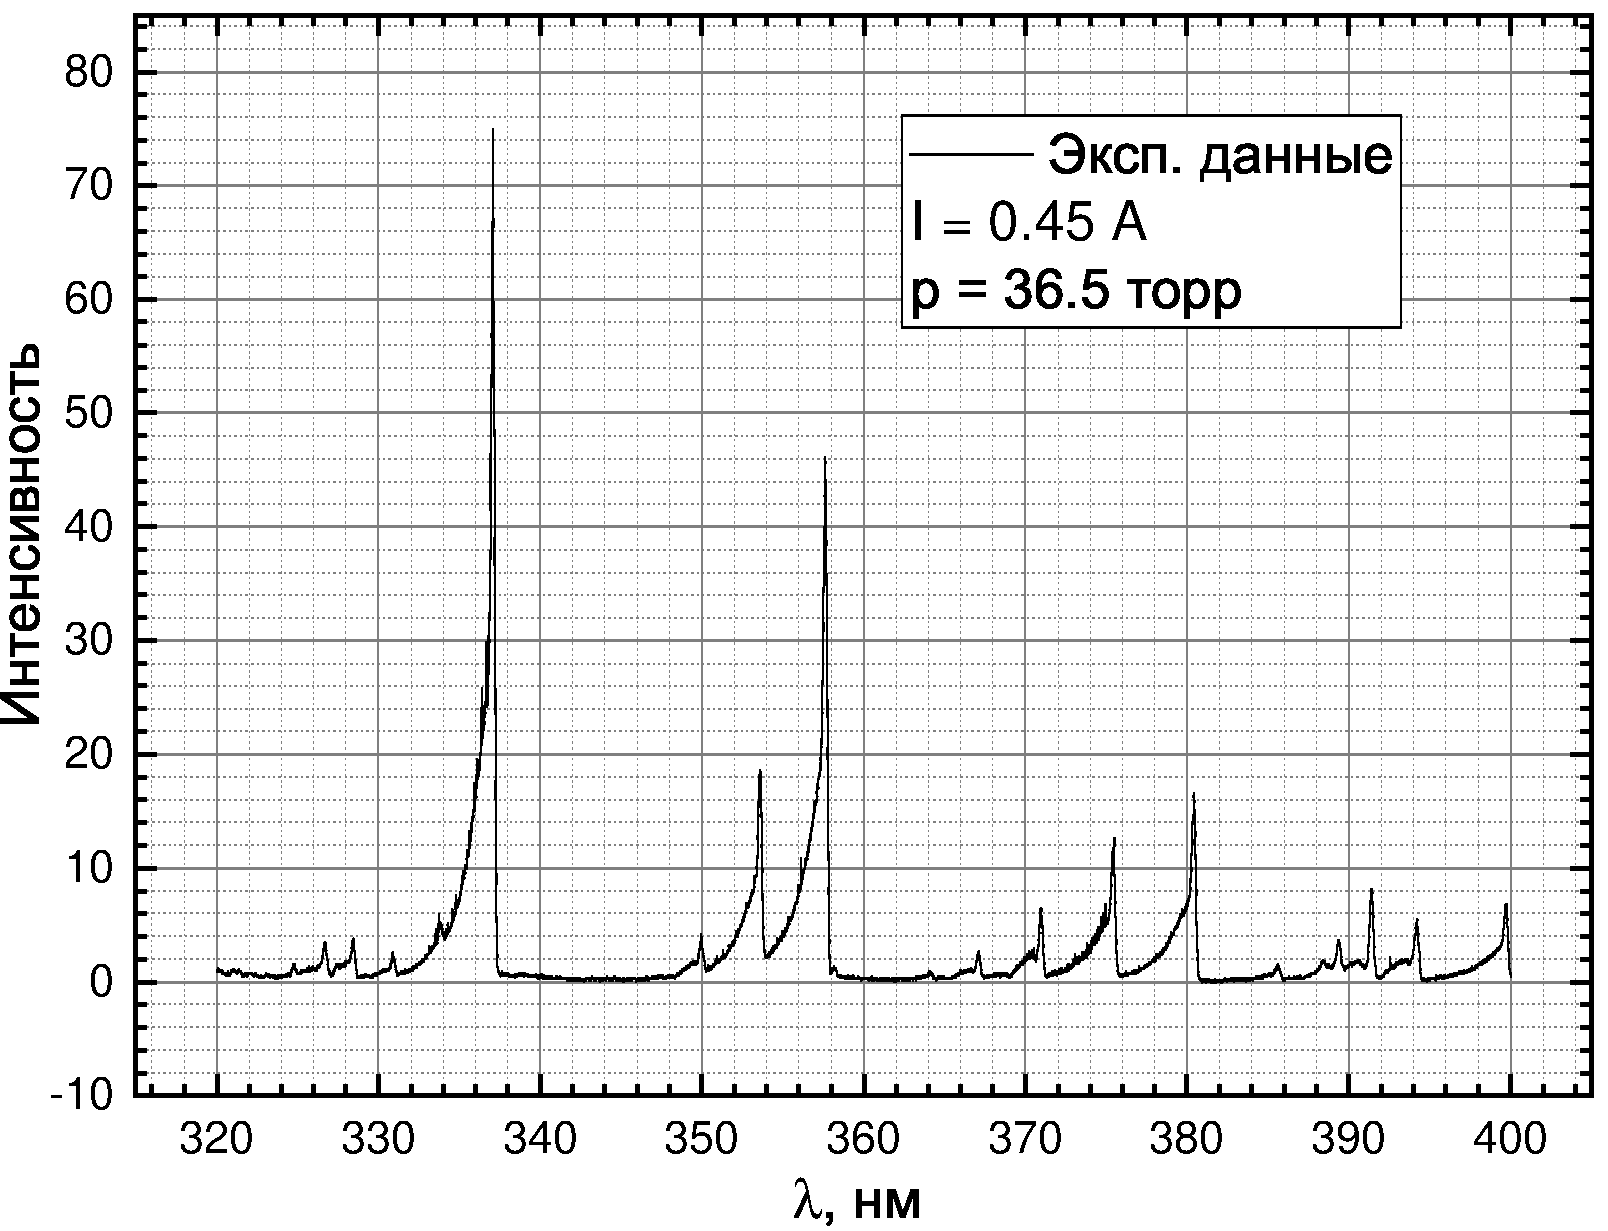
\includegraphics[width=\linewidth]{data/graph_I=0,45}
		\caption{Спектр при $I= 0.45$ А, $P$= 36.5 торр}
		\label{full_45}
	\end{minipage} 
	\hfill
	\begin{minipage}[H]{0.45\linewidth}
		\centering
		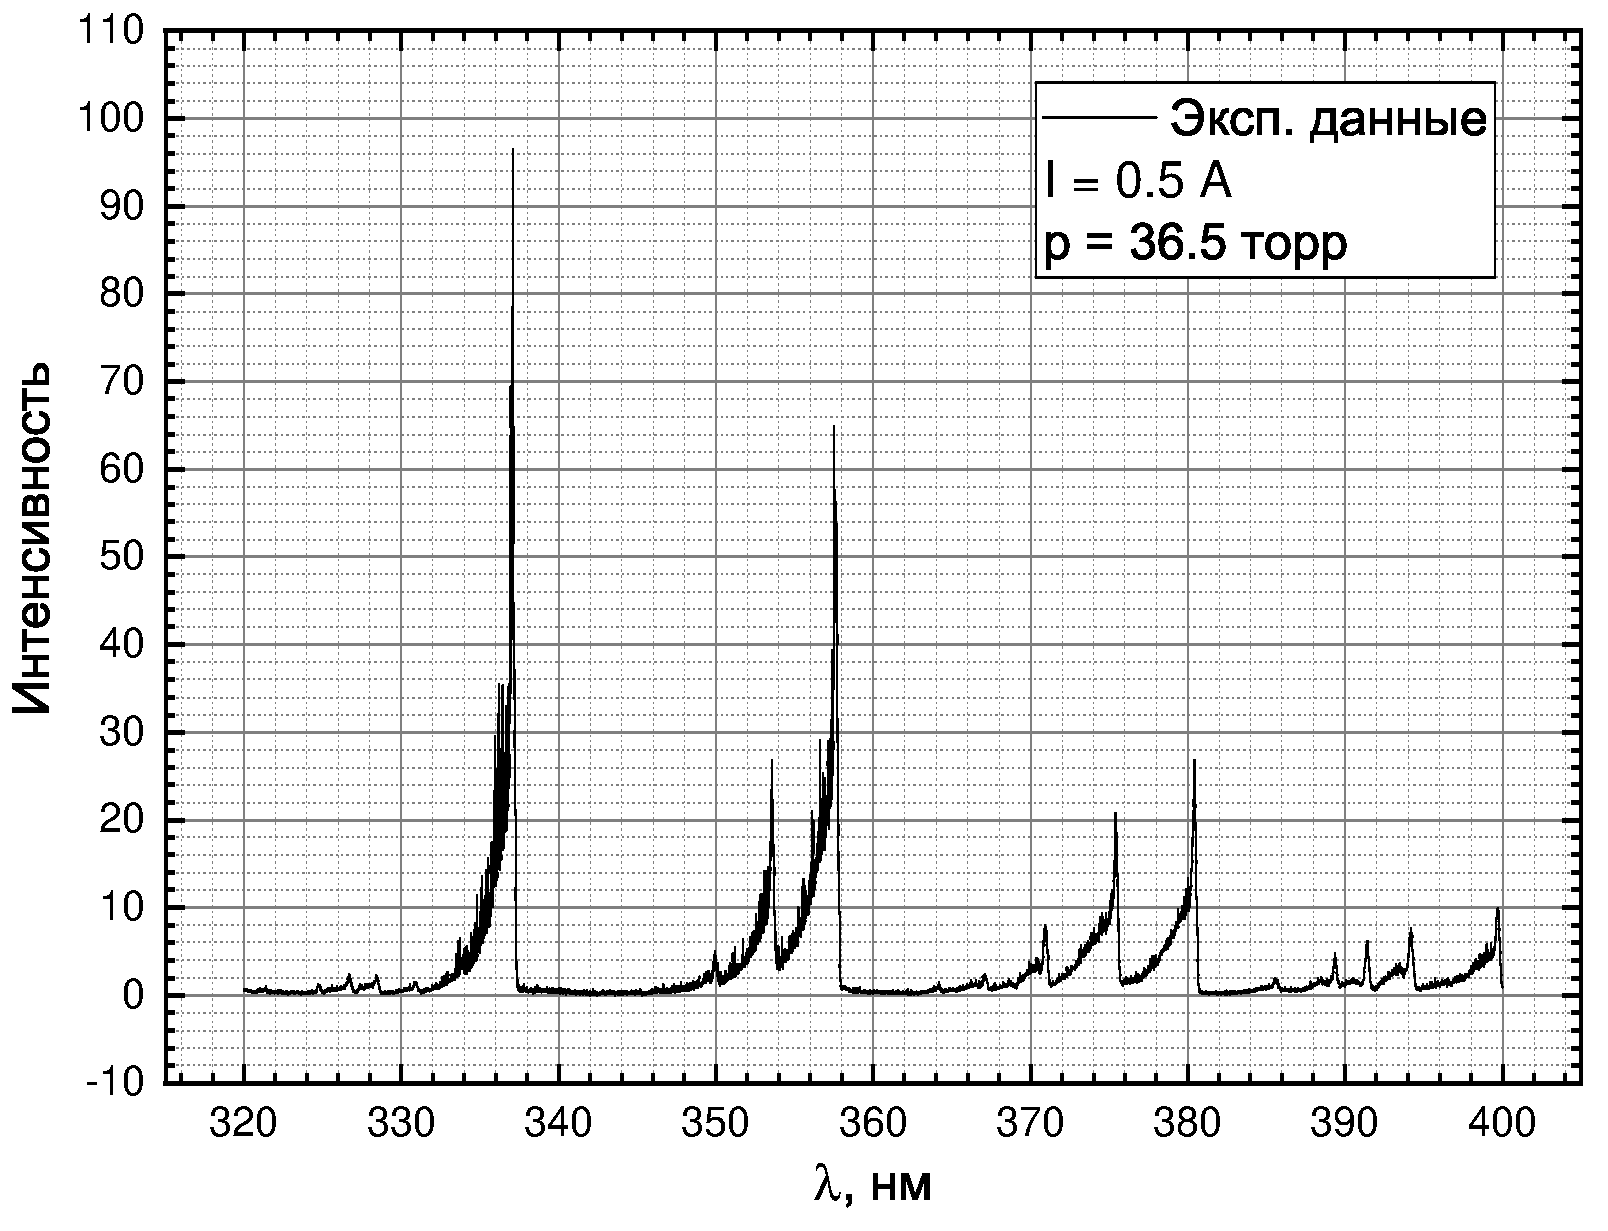
\includegraphics[width=\linewidth]{data/graph_I=0,50}
		\caption{Спектр при $I= 0.50 $ А, $P$= 36.5 торр}
		\label{full_50}
	\end{minipage}
	\begin{minipage}{0.45\linewidth}
		\centering
		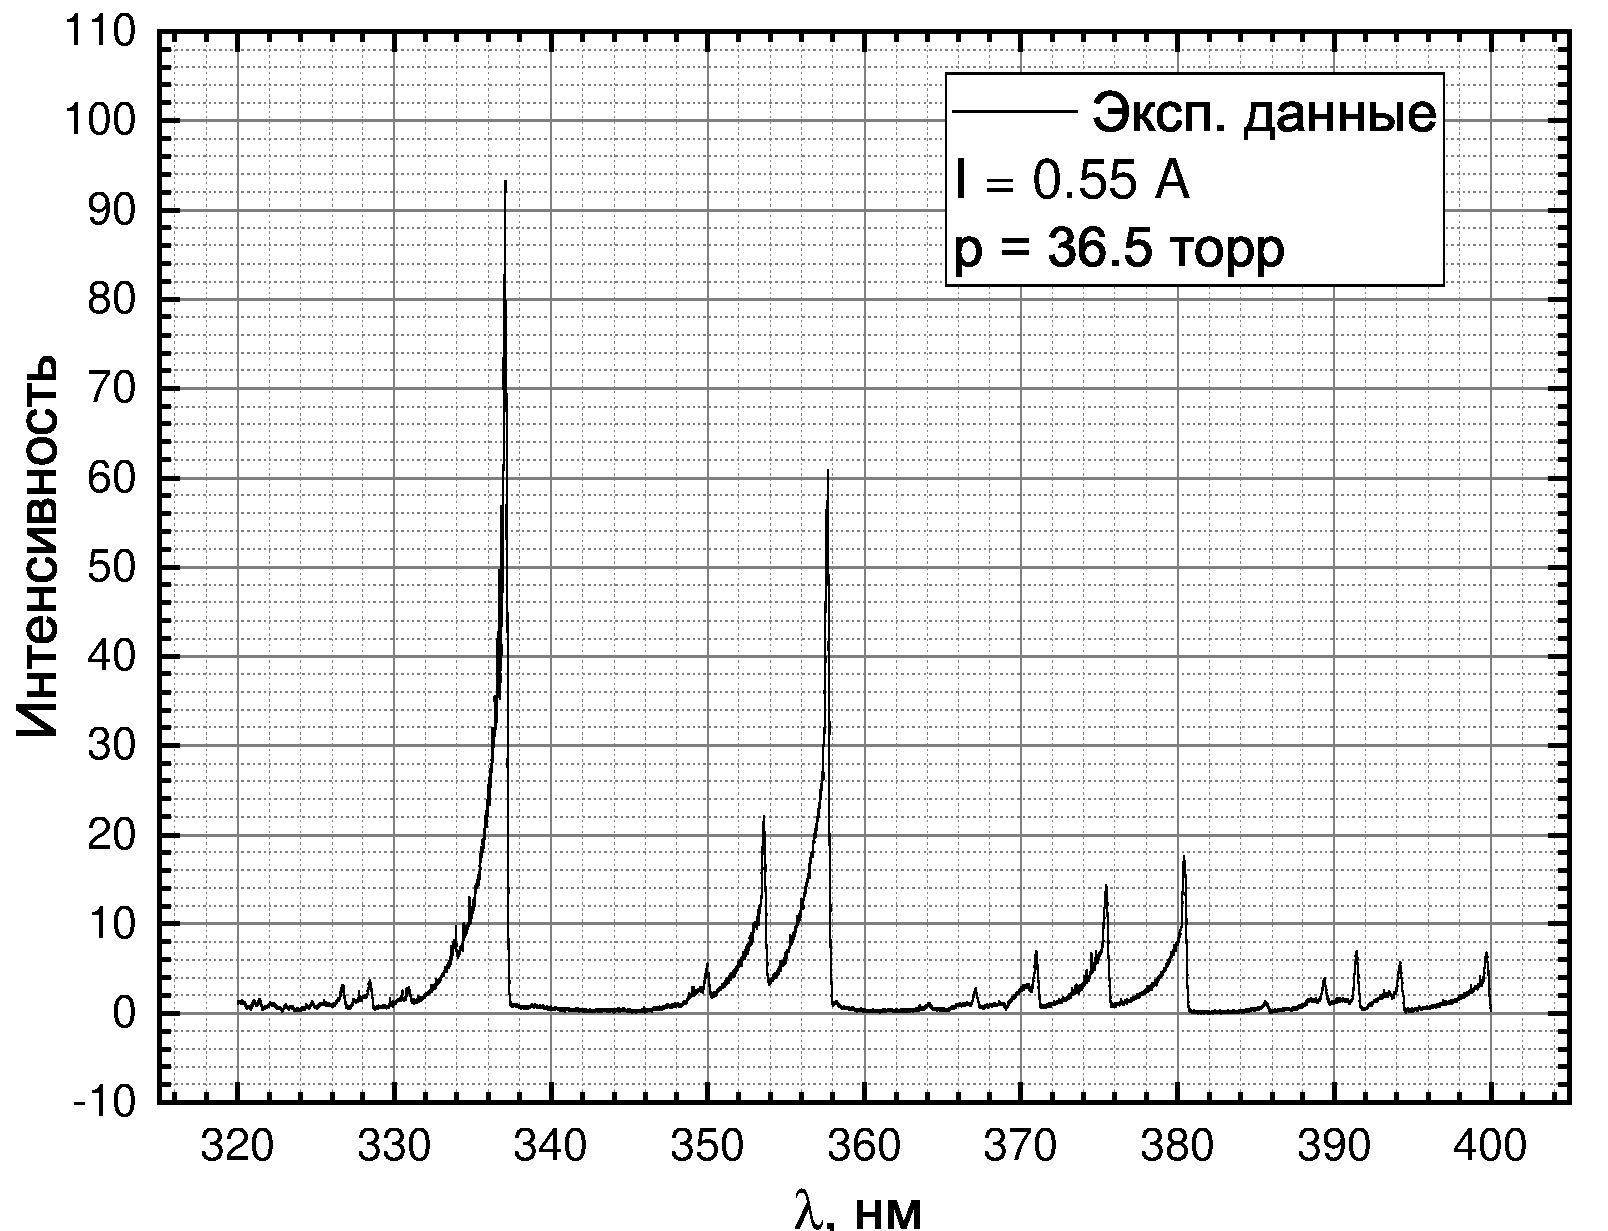
\includegraphics[width=\linewidth]{data/graph_I=0,55}
		\caption{Спектр при $I= 0.55 $ А, $P$= 36.5 торр}
		\label{full_55}	
	\end{minipage} 
	\hfill
	\begin{minipage}[H]{0.45\linewidth}
		\centering
		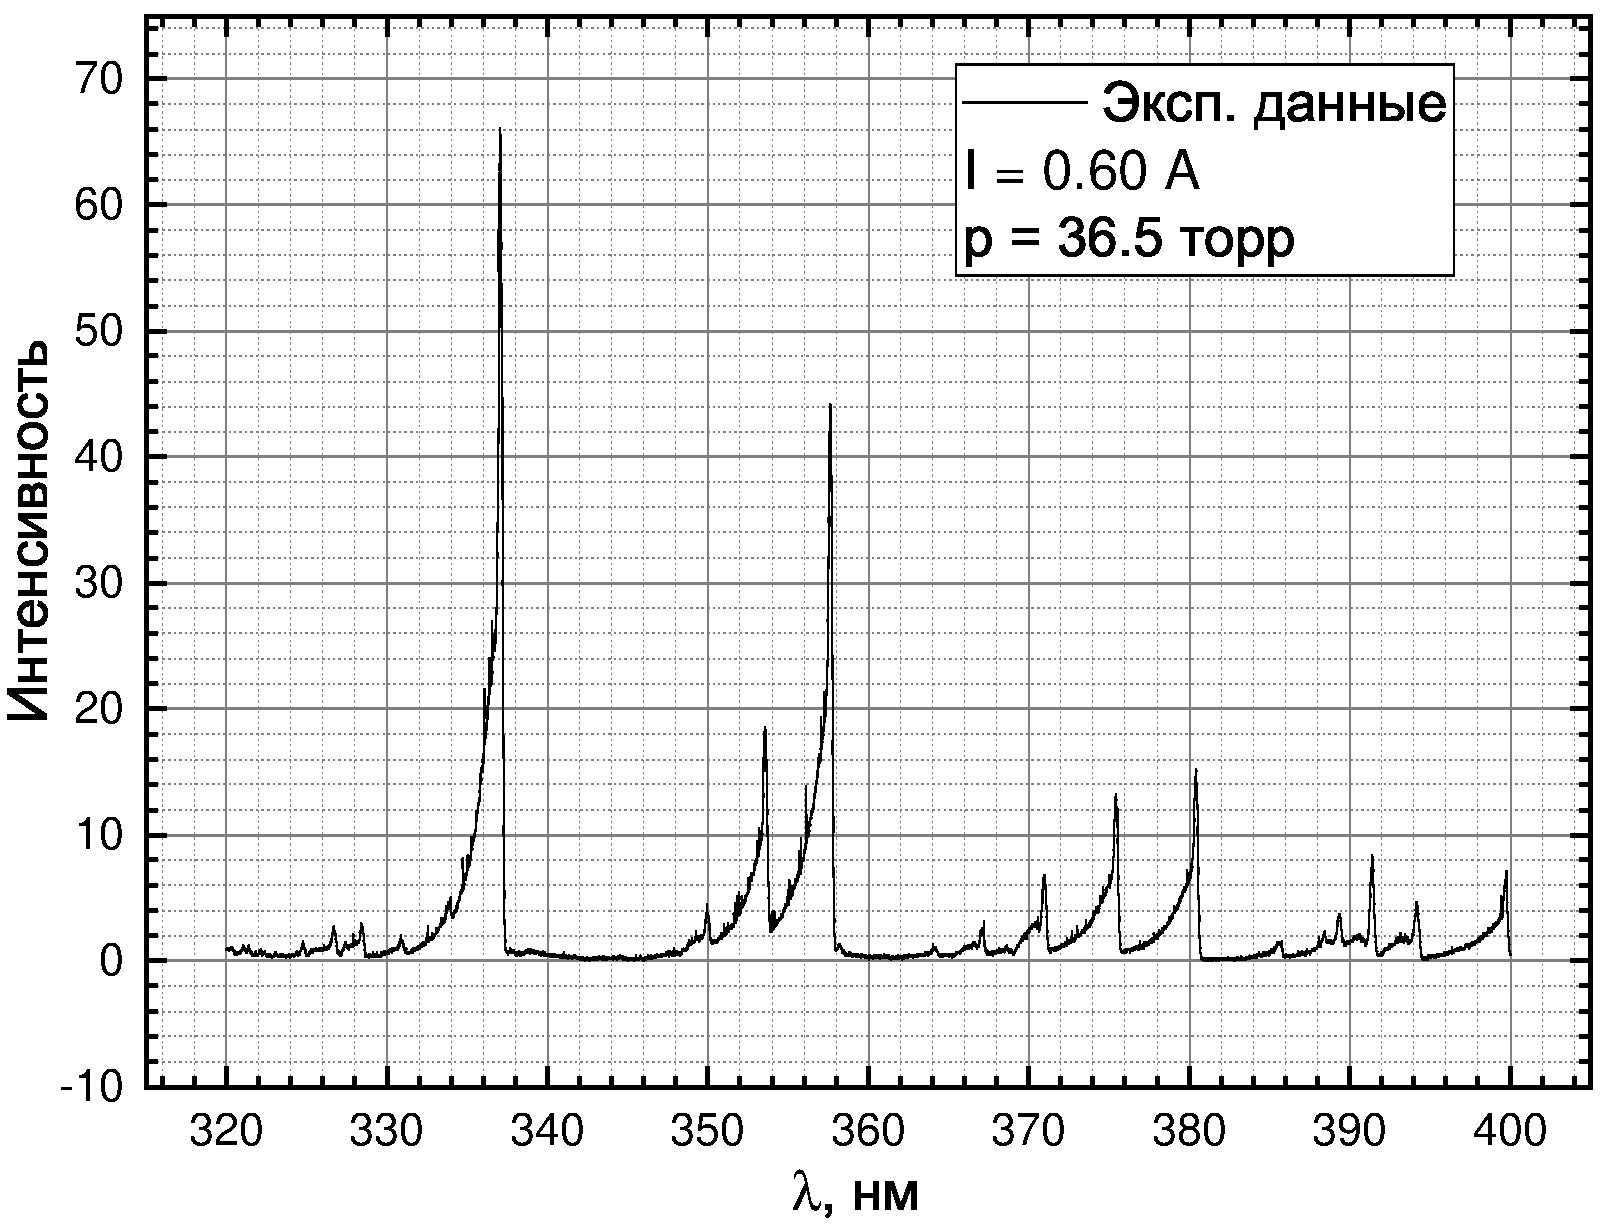
\includegraphics[width=\linewidth]{data/graph_I=0,60}
		\caption{Спектр при $I= 0.60 $ А, $P$= 36.5 торр}
		\label{full_60}
	\end{minipage}
	\begin{minipage}{0.45\linewidth}
		\centering
		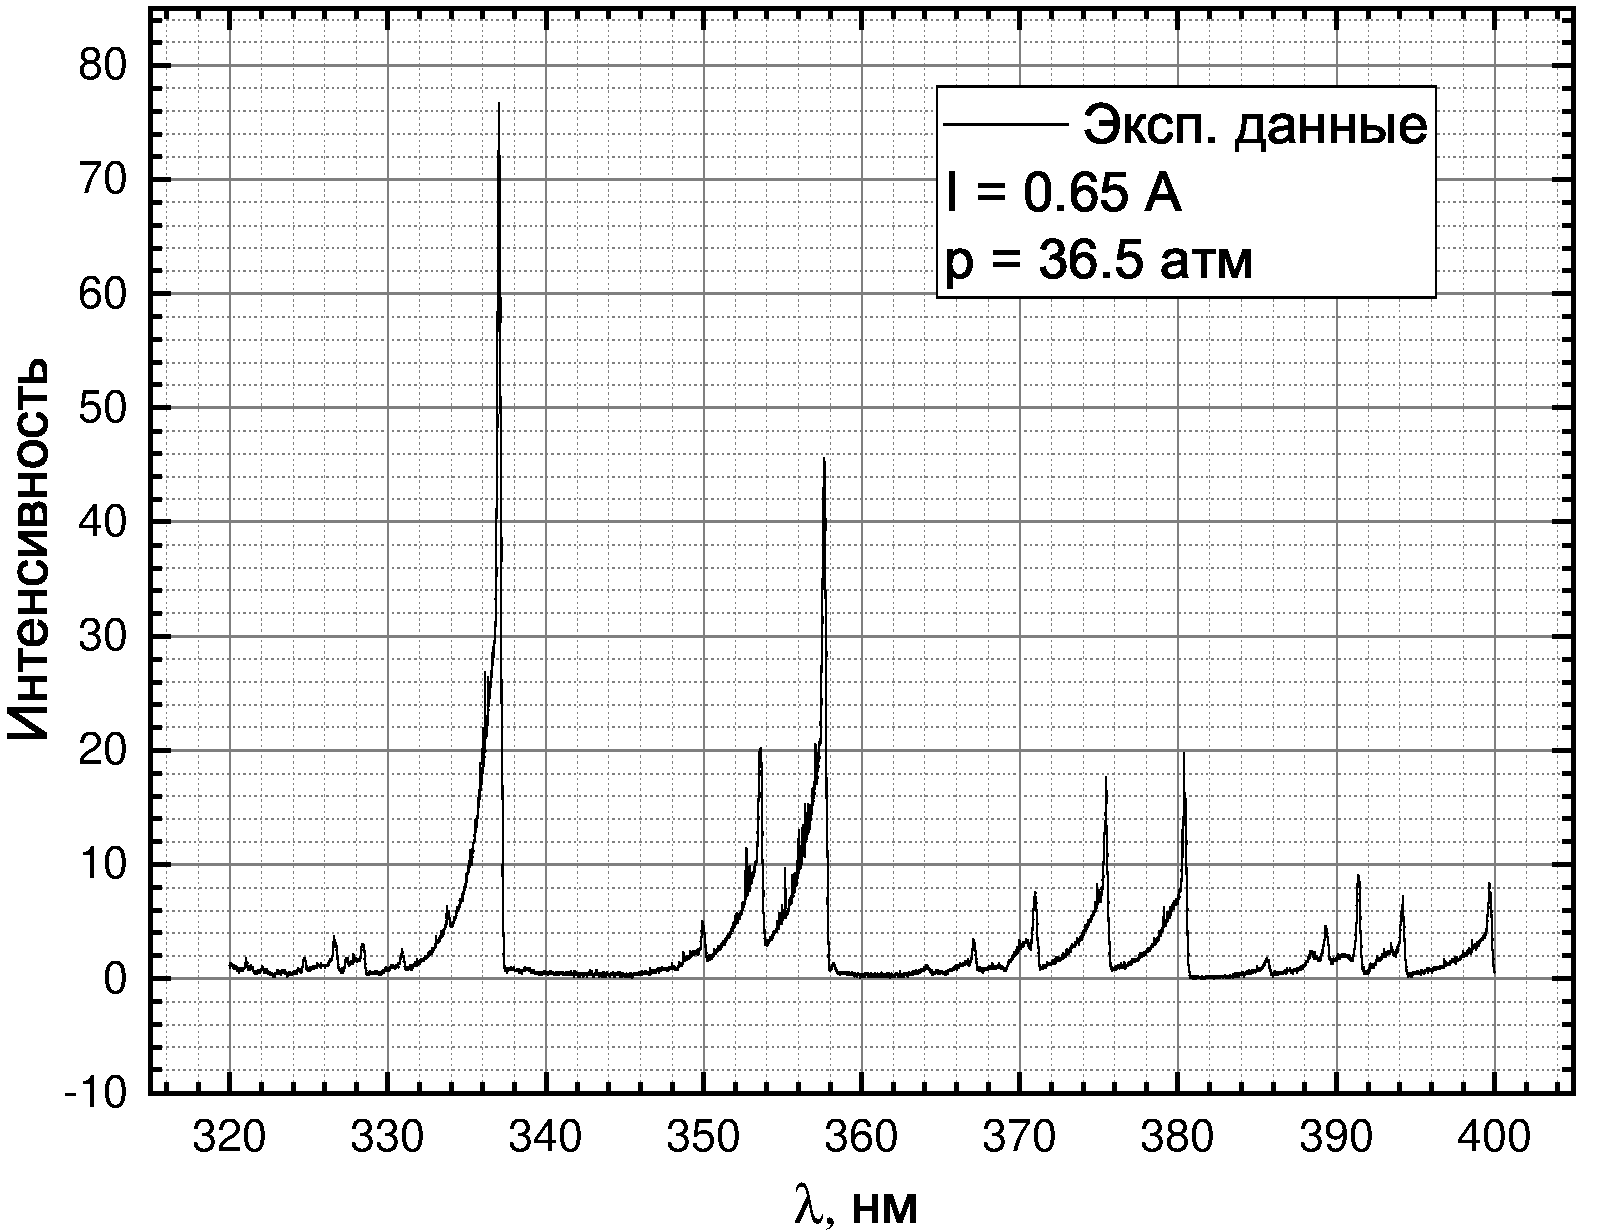
\includegraphics[width=\linewidth]{data/graph_I=0,65}
		\caption{Спектр при $I= 0.65 $ А, $P$= 36.5 торр}	
		\label{full_65}
	\end{minipage} 
	\hfill
\end{figure}

 % Table generated by Excel2LaTeX from sheet 'Лист1'
\begin{table}[H]
	\centering
	\caption{Соотнесение полос}
	\begin{tabular}{ | l | l | l | l | l | l | }
	\hline
	$I$, A & $\lambda$, нм & переход & $I$, A & $\lambda$, нм & переход \\
	\hline
	\hline
	0.65 & 337.03 & $0 \rightarrow 0$ & 0.60 & 337.06 & $0 \rightarrow 0$ \\ \hline
	0.65 & 357.61 & $0 \rightarrow 1$ & 0.60 & 357.64 & $0 \rightarrow 1$ \\ \hline
	0.65 & 353.60 & $1 \rightarrow 2$ & 0.60 & 353.55 &$ 1 \rightarrow 2$ \\ \hline
	0.65 & 349.92 & $2 \rightarrow 3$ & 0.60 & 349.93 & $2 \rightarrow 3$ \\ \hline
	0.65 & 380.37 & $0 \rightarrow 2$ & 0.60 & 380.42 & $0 \rightarrow 2$ \\ \hline
	0.65 & 375.44 & $1 \rightarrow 3$ & 0.60 & 375.42 & $1 \rightarrow 3$ \\ \hline
	0.65 & 370.97 & $2 \rightarrow 4$ & 0.60 & 370.98 & $2 \rightarrow 4$ \\ \hline
	0.65 & 367.06 & $3 \rightarrow 5$ & 0.60 & 367.19 & $3 \rightarrow 5$ \\ \hline
	\end{tabular}
	\label{tab:polosi}%
\end{table}%

\subsection{Вычисление вращательной температуры}
Для вычисления вращательной температуры выберем участок неразрешенной
вращательной структуры и прологарифмируем его. По наклону прямой зависимости $\lg I=f(\lambda)$ , используя рассчитанную
зависимость тангенса угла наклона от значения вращательной температуры, определим значение вращательной температуры в центральной части разряда. Результаты занесем в таблицу \ref{tab:T_rot}.

\begin{table}[H]
	\centering
	\caption{Расчет вращательной температуры по угловому коэффициенту}
	\begin{tabular}{|c|c|}
		\hline 
		$I$, A & $T_\text{rot}$, K \\ 
		\hline 
		0.45 & 1000 \\ 
		\hline 
		0.50 & 1382 \\ 
		\hline 
		0.55 & 1210 \\ 
		\hline 
		0.6 & 1209 \\ 
		\hline 
		0.65 & 1234 \\ 
		\hline 
	\end{tabular} 
	\label{tab:T_rot}
\end{table}

\begin{figure}[H]
	\begin{minipage}{0.45\linewidth}
		\centering
		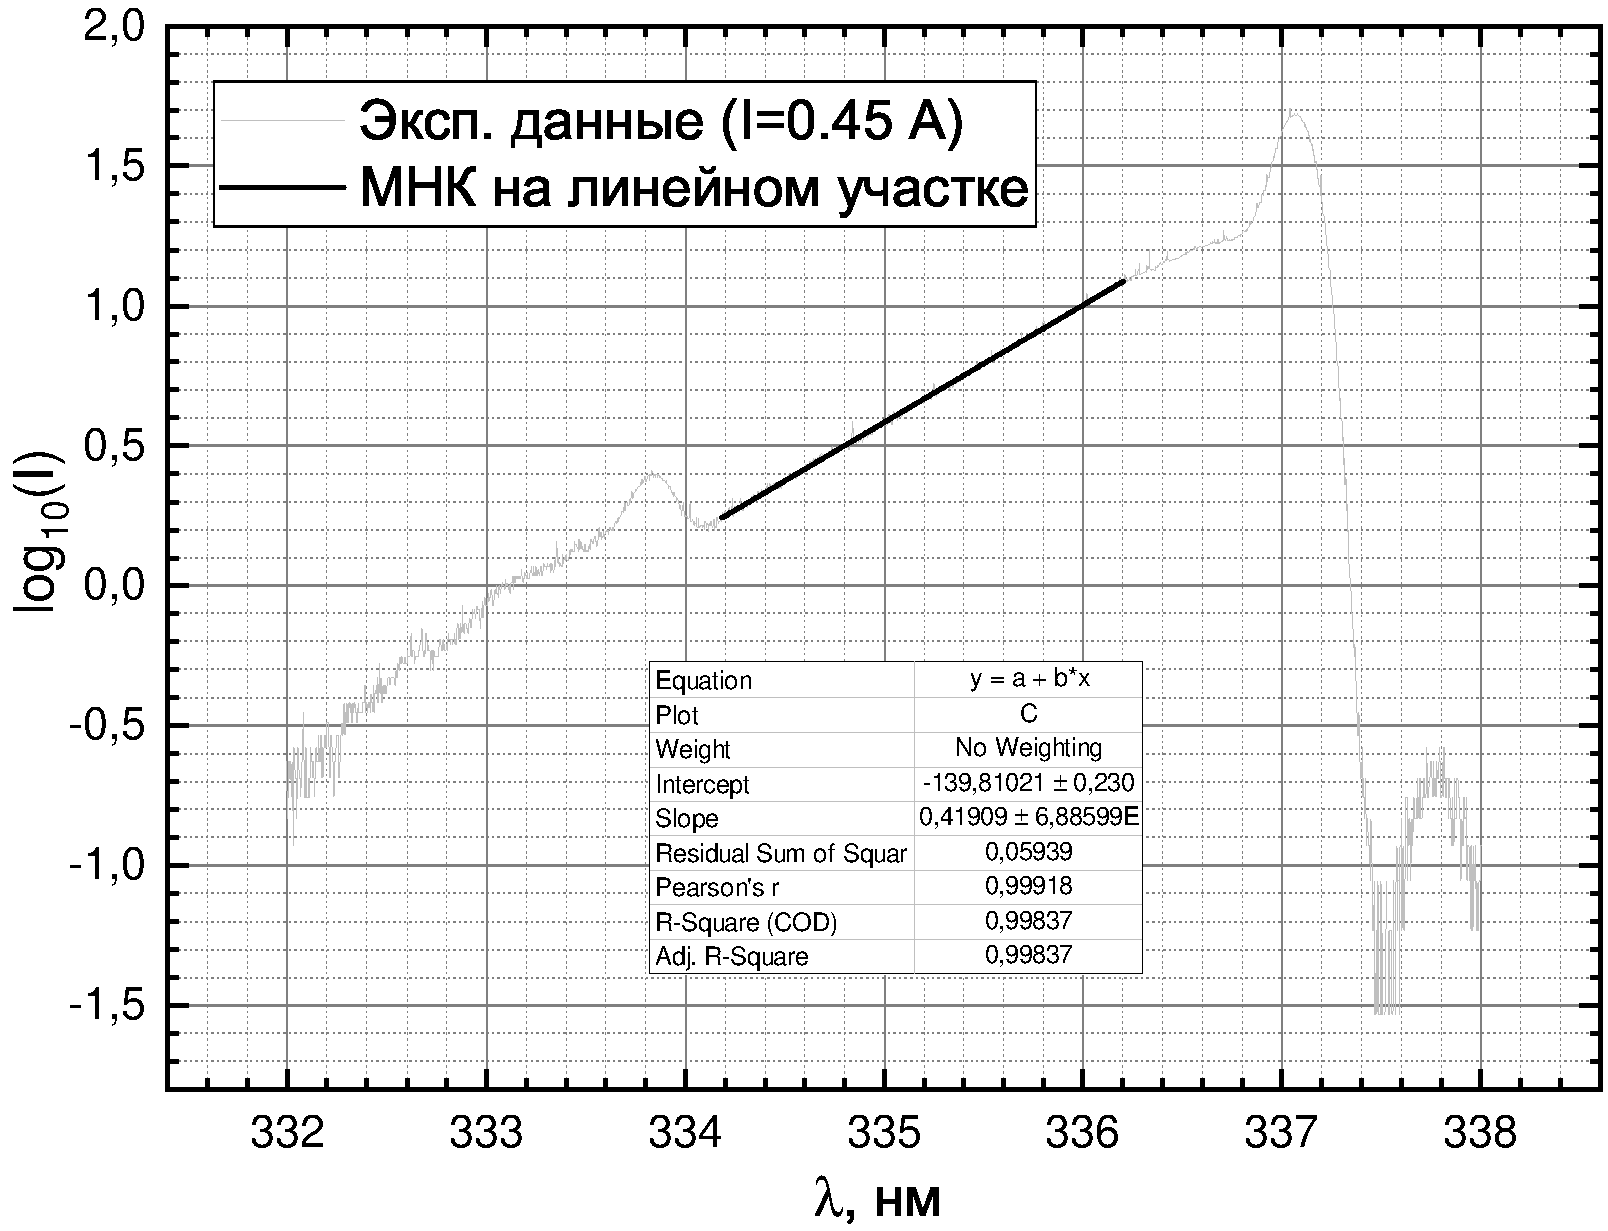
\includegraphics[width=\linewidth]{data/graph_I=0,45_polosa}
		\caption{Спектр при $I= 0.45$ А, $P$= 36.5 торр}
		\label{polosa_45}
	\end{minipage} 
	\hfill
	\begin{minipage}[H]{0.45\linewidth}
		\centering
		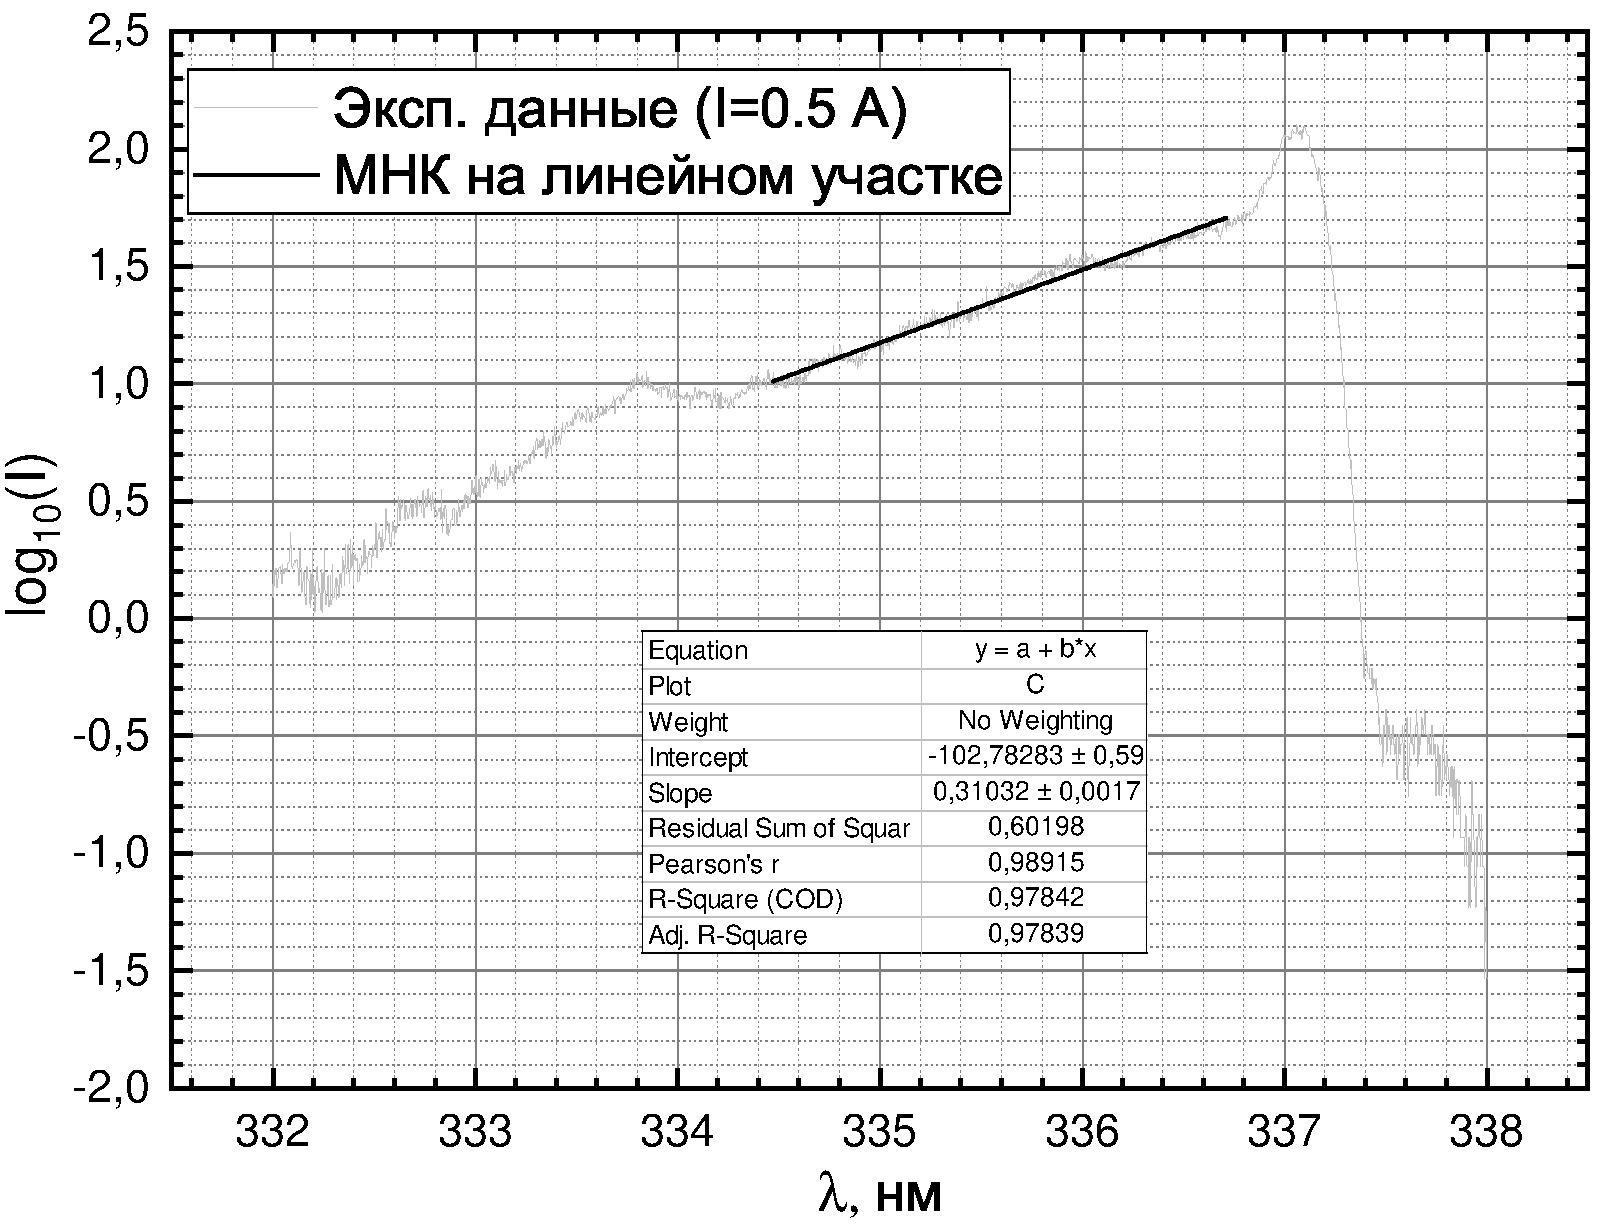
\includegraphics[width=\linewidth]{data/graph_I=0,50_polosa}
		\caption{Спектр при $I= 0.50 $ А, $P$= 36.5 торр}
		\label{polosa_50}
	\end{minipage}
	\begin{minipage}{0.45\linewidth}
		\centering
		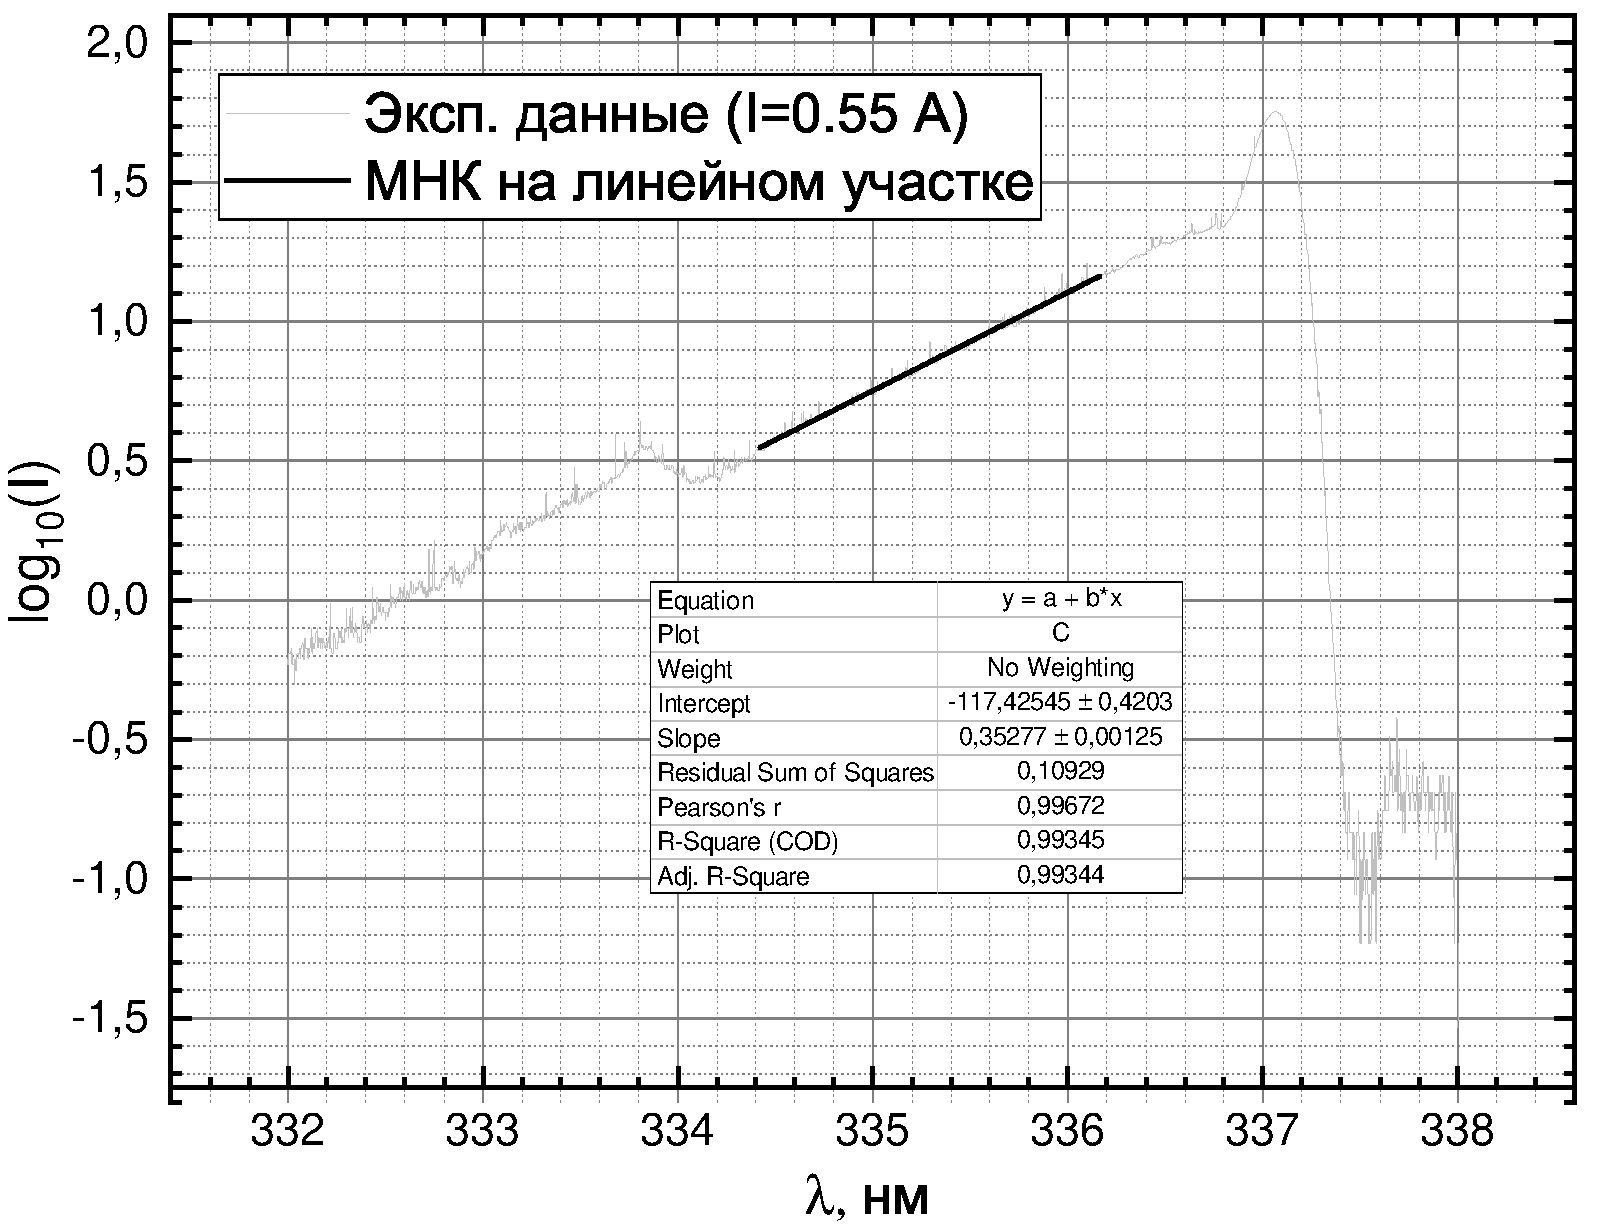
\includegraphics[width=\linewidth]{data/graph_I=0,55_polosa}
		\caption{Спектр при $I= 0.55 $ А, $P$= 36.5 торр}
		\label{polosa_55}	
	\end{minipage} 
	\hfill
	\begin{minipage}[H]{0.45\linewidth}
		\centering
		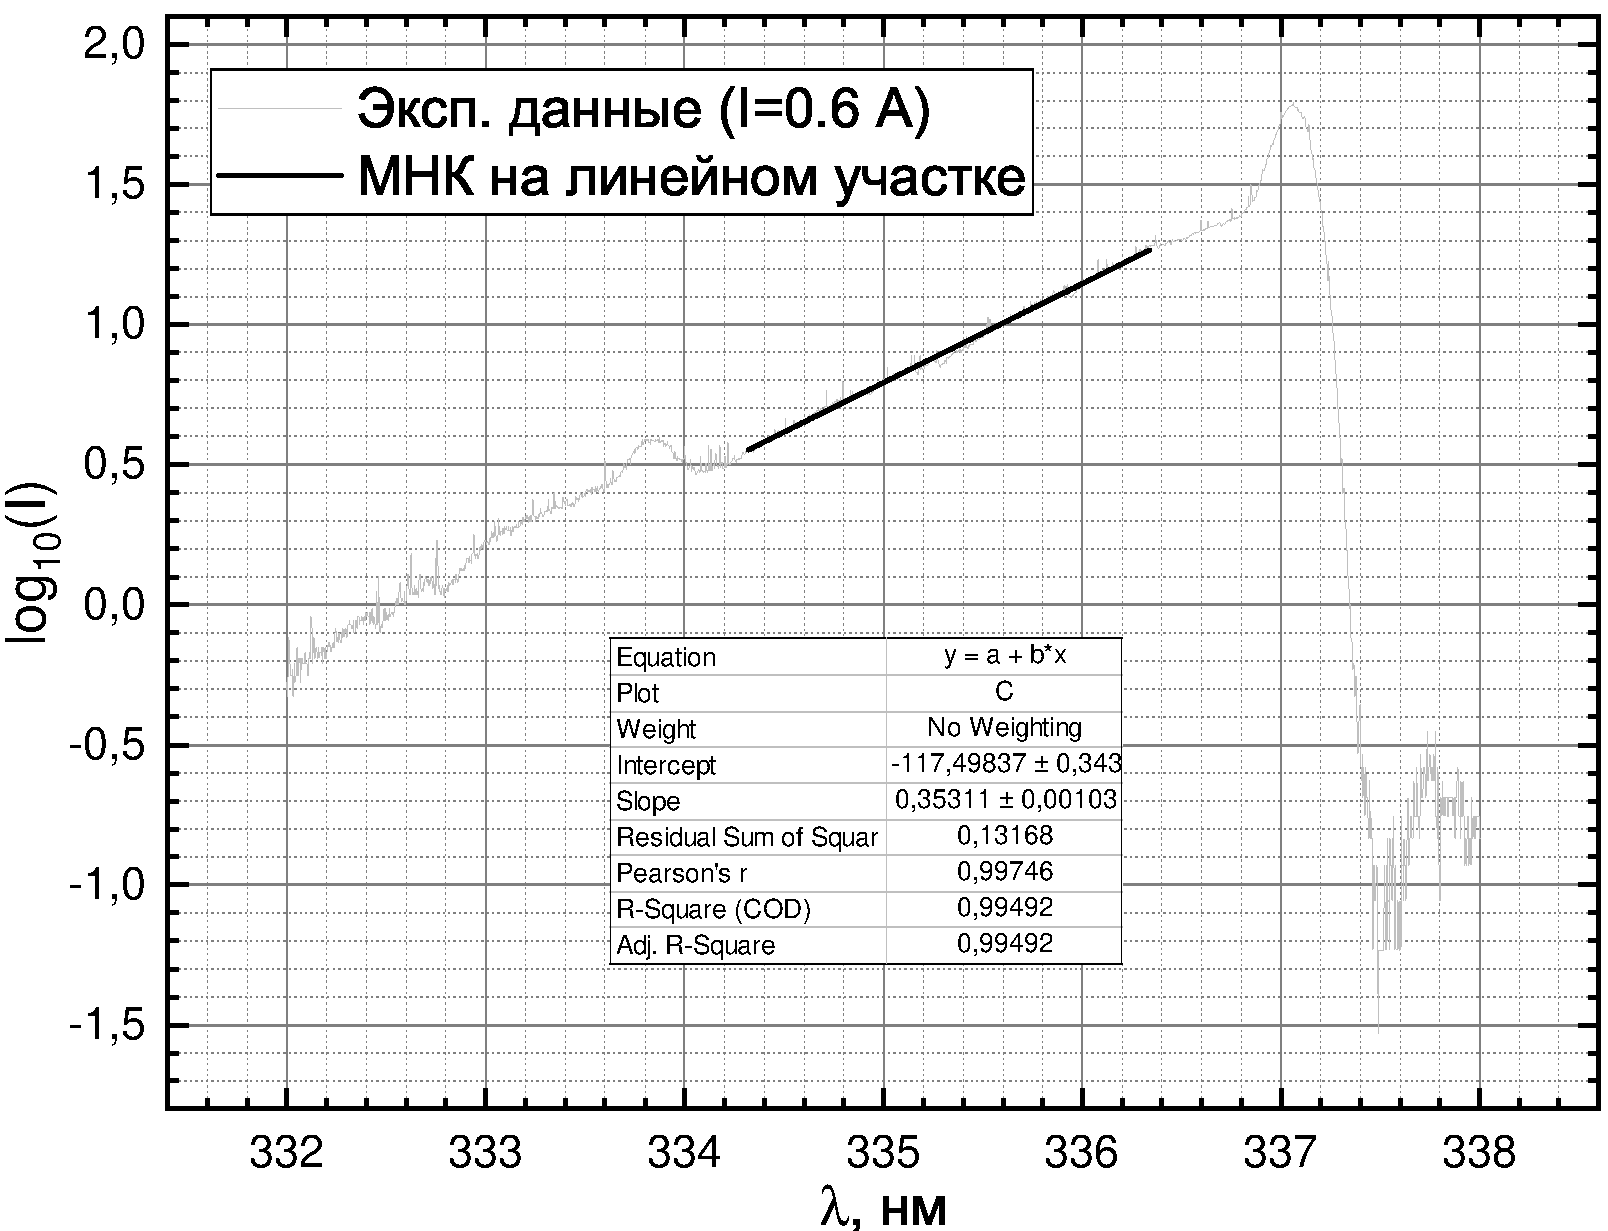
\includegraphics[width=\linewidth]{data/graph_I=0,60_polosa}
		\caption{Спектр при $I= 0.60 $ А, $P$= 36.5 торр}
		\label{polosa_60}
	\end{minipage}
	\begin{minipage}{0.45\linewidth}
		\centering
		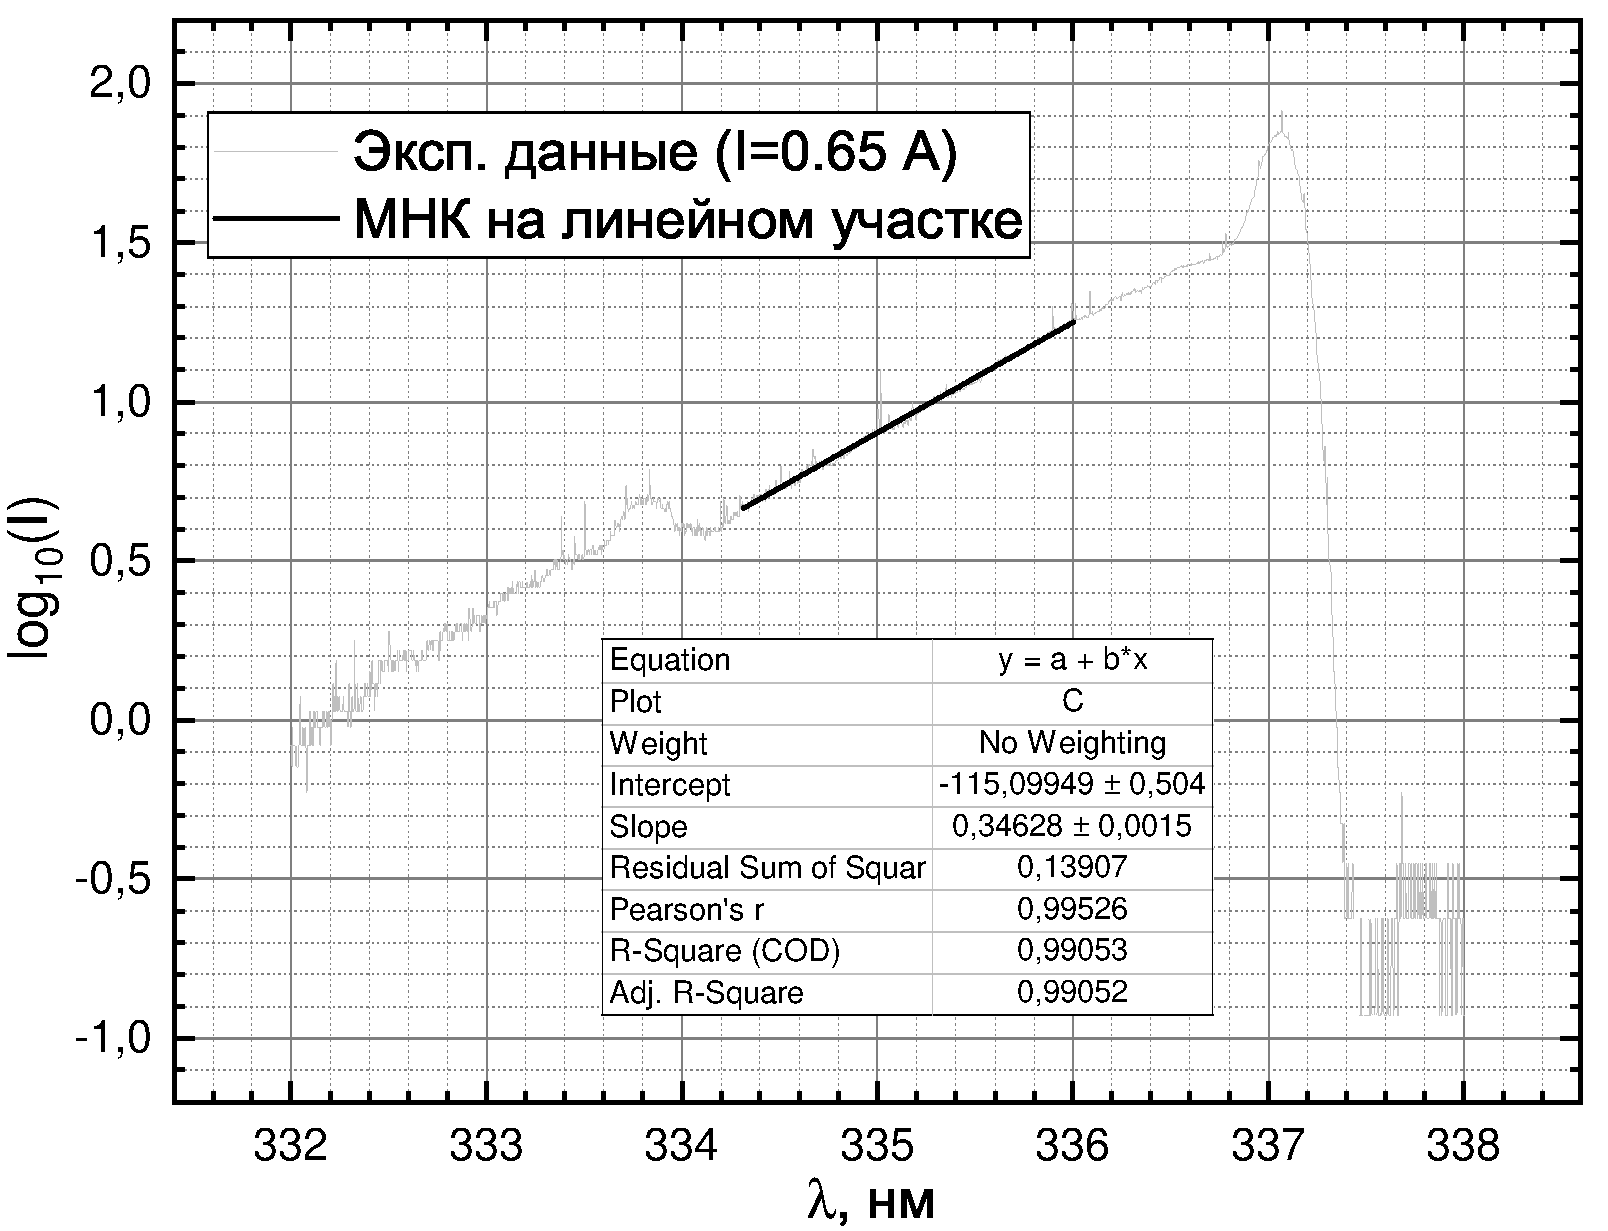
\includegraphics[width=\linewidth]{data/graph_I=0,65_polosa}
		\caption{Спектр при $I= 0.65 $ А, $P$= 36.5 торр}	
		\label{polosa_65}
	\end{minipage} 
	\hfill
\end{figure}
%\newpage
\section{Заключение}
В данной работе рассматривался спектр поглощения молекулы йода. Были получены молекулярные константы, построен потенциал Морзе для возбужденного состояния молекулы $\text{I}_2$.

% TODO: точно у нас так же?
Оказалось, что самый близкий к табличному результат дал метод линейной экстраполяции. 

Анализ спектров при разных ширинах щели показывает, что с уменьшением размера щели увеличивается разрешающая способность прибора. Электронно-колебательную структуру спектра мы начинаем разрешать при ширине щели около 0.5 нм.

Анализ спектра широкого диапазона показывает, что есть 2 характерные области $v''$--прогрессий, а при уменьшении возбуждающей длины волны молекула начинает диссоциировать.

\begin{comment}
\begin{thebibliography}{1}
\bibitem{1}
ЯМР-релаксаця : учебно-методическое пособие / сост.: А.
М. Перепухов, А.В. Максимычев, О.В. Кишенков, А.Ю. Куксин –
М.: МФТИ, 2015.
\end{thebibliography}
\end{comment}



%\bibliography{mybibliography}
%\bibliographystyle{gost705}

\end{document}
